\documentclass[12pt,a4paper,dvipsnames,usenames]{beamer}
\usepackage{url}
\usepackage{xcolor}
\usepackage{amsmath,varwidth,slashed}
%\usepackage[utf8]{inputenc}
\usepackage[T1]{fontenc}
\usepackage{tikz,xparse}
\usepackage[normalem]{ulem}
\usepackage{appendixnumberbeamer}
\usepackage{pdfpages}

% -------------------------- %
% Standard LaTeX definitions %
% -------------------------- %

\DeclareGraphicsExtensions{.pdf}
\renewcommand\textbullet{\ensuremath{\bullet}}

% ----------------------------------- %
% Various tikz styles and definitions %
% ----------------------------------- %

\usetikzlibrary{calc,intersections,positioning,matrix,chains,scopes}
\usetikzlibrary{decorations.pathmorphing,decorations.pathreplacing,shapes}
\newcommand{\tikzmark}[1]{\tikz[overlay,remember picture] \node (#1) {};}

\tikzumlset{fill class=RoyalBlue!20}

\tikzstyle{startnode} = [circle, draw, fill=Bittersweet!20, minimum size=10pt, inner sep = 0]
\tikzstyle{stopnode} = [startnode]
\tikzstyle{process} = [rectangle, minimum width=2cm, minimum height=.7cm, text centered, draw, fill=OliveGreen!20, align=center, font=\scriptsize]
\tikzstyle{dangerprocess} = [process, fill=BrickRed!20, draw=BrickRed, thick]
\tikzstyle{flowarrow} = [->, >=stealth, thick]

% ---------------------------------- %
% My default listings C++ code style %
% ---------------------------------- %

\lstset{%
  language=C++, basicstyle=\scriptsize\ttfamily, 
  keywordstyle=\color{OliveGreen}, identifierstyle=\color{RoyalBlue}, 
  commentstyle=\color{Brown}, stringstyle=\color{Bittersweet}, showstringspaces=false,  
  breaklines=true, prebreak=\mbox{{\color{Bittersweet}\tiny\ $\hookleftarrow$}}, 
  postbreak=\mbox{{\color{Bittersweet}\tiny$\to$\ }}, tabsize=5,
  morekeywords={%
    MyClass,unique_ptr,shared_ptr,weak_ptr,auto_ptr,
    make_unique, make_shared, default_delete,
    dynamic_pointer_cast, const_pointer_cast,
    scoped_ptr,QSharedPointer,QScopedPointer,QWeakPointer,
    ftring, SmartPtr, Shape, Circle, ShapeFactory, CircleFactory,
    Derived, Base
  }
}

\def\inline{\lstinline[basicstyle=\ttfamily\normalsize]}

% ---------------------------------------------------------------------------------------------------- %
% Various command for inline code instead of lstinline so that I don't have to update the keyword list %
% ---------------------------------------------------------------------------------------------------- %

\newcommand{\object}[1]{{\ttfamily \color{OliveGreen}#1}}
\newcommand{\function}[1]{{\ttfamily \color{RoyalBlue}#1}}
\newcommand{\std}[1]{{\ttfamily {\color{RoyalBlue} std::}{\color{OliveGreen}#1}}}
\newcommand{\boost}[1]{{\ttfamily {\color{RoyalBlue} boost::}{\color{OliveGreen}#1}}}

\newcommand{\uniqueptr}{\std{unique\_ptr}}
\newcommand{\sharedptr}{\std{shared\_ptr}}
\newcommand{\weakptr}{\std{weak\_ptr}}
\newcommand{\autoptr}{\std{auto\_ptr}}

% The base16 colour scheme?
\definecolor{sbase03}{HTML}{002B36}
\definecolor{sbase02}{HTML}{073642}
\definecolor{sbase01}{HTML}{586E75}
\definecolor{sbase00}{HTML}{657B83}
\definecolor{sbase0}{HTML}{839496}
\definecolor{sbase1}{HTML}{93A1A1}
\definecolor{sbase2}{HTML}{EEE8D5}
\definecolor{sbase3}{HTML}{FDF6E3}
\definecolor{syellow}{HTML}{B58900}
\definecolor{sorange}{HTML}{CB4B16}
\definecolor{sred}{HTML}{DC322F}
\definecolor{smagenta}{HTML}{D33682}
\definecolor{sviolet}{HTML}{6C71C4}
\definecolor{sblue}{HTML}{268BD2}
\definecolor{scyan}{HTML}{2AA198}
\definecolor{sgreen}{HTML}{859900}

\definecolor{Tropiteal}{RGB}{0,168,198}
\definecolor{TealDrop}{RGB}{64,192,203}
\definecolor{WhiteTrash}{RGB}{249,242,231}
\definecolor{AtomicBikini}{RGB}{174,226,57}
\definecolor{FeebleWeek}{RGB}{143,190,0}
\definecolor{ICantExpress}{RGB}{28,20,13}
\definecolor{Marty}{RGB}{250,42,0}

\colorlet{ColourBase}{Tropiteal}
\colorlet{ColourHl1}{Marty}
\colorlet{ColourHl2}{FeebleWeek}
\colorlet{ColourHl3}{TealDrop}
\colorlet{ColourDark}{ICantExpress}
\colorlet{ColourDark2}{Tropiteal}


\usetheme{metropolis}

\setbeamercolor{alerted text}{%
  fg=bazelGreen
}

\setbeamercolor{example text}{%
  fg=mLightBrown
}

\setbeamercolor{frametitle}{%
  use=normal text,
  fg=normal text.bg,
  bg=bazelGreen
}

\lstset{%
  basicstyle=\ttfamily\lst@ifdisplaystyle\fontsize{9pt}{9pt}\selectfont\fi,
  keywordstyle=\color{sgreen}, identifierstyle=\color{sblue}, 
  commentstyle=\color{sbase1}, stringstyle=\color{sorange},
  numberstyle=\color{sviolet}, showstringspaces=false,  
  breaklines=true,
  tabsize=5,
}

\lstalias[]{gnumake}[gnu]{make}

\newcommand{\dimtext}[2]%
{
  { \transparent{0.7}
  \begin{tikzpicture}[overlay, remember picture]
    \fill[white] ( #1 -| current page.north west) -- ++(0,.8em) -- ++(\paperwidth,0) -- (#2 -| current page.north east)
   -- ++(0,-.5em) -- ++(-\paperwidth,0) -- cycle;
  \end{tikzpicture}
  }
}

\newcommand{\specialcell}[2][c]{%
  \begin{tabular}
    [#1]{@{}c@{}}#2
  \end{tabular}
}

\newcommand{\tikzmark}[1]{\tikz[overlay,remember picture] \coordinate (#1);}

\newcommand{\qmat}{\ensuremath{Q_{\mathrm{uark}}}}
\newcommand{\mathfont}{\fontsize{10pt}{12pt}}
\newcommand{\minus}{\scalebox{0.75}[1.0]{$-$}}
\newcommand{\sectionframe}{%
  \addtocounter{framenumber}{-1}%
  \frame[plain]{\begin{center}\LARGE \color{beameralert} \insertsection\end{center}}}

\newcommand{\breakline}{%
  \begin{center} \begin{tikzpicture}
      \draw[beamerprimary] ({-0.5 * \textwidth},0) -- ({0.5 * \textwidth},0);
      \node[inner sep=0, minimum size=7pt, fill=white,circle] {};
      \node[inner sep=0, minimum size=4pt, draw=beamerprimary,circle] {};
      \node[inner sep=0, minimum size=1pt, fill=beamerprimary,circle] {};
  \end{tikzpicture} \end{center}
}


\title{Analytical computations of an effective lattice theory for heavy quarks}
\author{Aleksandra R. Glesaaen\texorpdfstring{\\[2pt]\small Mathias Neuman, Owe Philipsen}{}}
\institute{\texorpdfstring{
\includegraphics[scale=0.08]{Figs/GU-Logo-blau-CMYK.pdf}}{Goethe University}}
\date{Bielefeld University, October 27th 2015}

\begin{document}

\setlength{\abovedisplayskip}{0pt}
\setlength{\belowdisplayskip}{0pt}

\begin{frame}[plain]
  \titlepage
\end{frame}

\setcounter{framenumber}{0}

\begin{frame}[plain]
  \tableofcontents
\end{frame}

\section{Introduction}
\sectionframe

\begin{frame}
  \frametitle{Putative QCD phase diagram}

  {\centering%
    \only<1|handout:1>{\includegraphics[scale=1.5]{Figs/phasediag1.pdf}}%
    \only<2|handout:2>{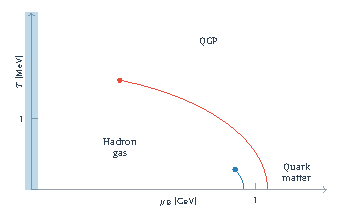
\includegraphics[scale=1.5]{Figs/phasediag2.pdf}}%
    \only<3|handout:3>{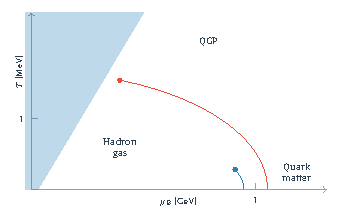
\includegraphics[scale=1.5]{Figs/phasediag3.pdf}}%
    \only<4|handout:4>{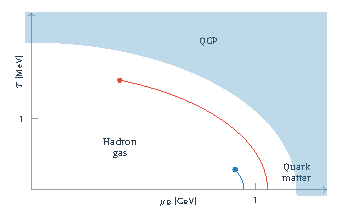
\includegraphics[scale=1.5]{Figs/phasediag4.pdf}}%
    \only<5|handout:5>{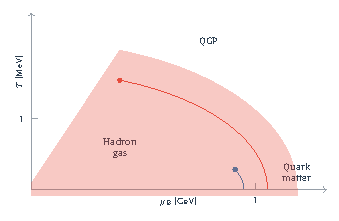
\includegraphics[scale=1.5]{Figs/phasediag5.pdf}}%
    \par
  }

  \begin{overlayarea}{\textwidth}{3em}
  \only<1|handout:1>{
  \begin{itemize}
    \item Different approaches can access different regions
  \end{itemize}}
  \only<2|handout:2>{
  \begin{itemize}
    \item Naive reach of Lattice QCD
  \end{itemize}}
  \only<3|handout:3>{
  \begin{itemize}
    \item Lattice QCD with additional methods \\ (analytic continuation, taylor expansions, reweighting,...)
  \end{itemize}}
  \only<4|handout:4>{
  \begin{itemize}
    \item Perturbation theory of QCD
  \end{itemize}}
  \only<5|handout:5>{
  \begin{itemize}
    \item Region currently not accessible from first principles with traditional methods
  \end{itemize}}
  \end{overlayarea}

\end{frame}

\begin{frame}
  \frametitle{The cold and dense}

  \begin{center}
    \includegraphics[scale=1.5]{Figs/cold_dense_phase_diag.pdf}
  \end{center}

  \vspace*{-.5cm}

  \begin{block}{Lattice requirements}
    \begin{itemize} \color{LightUIBase}
      \item $a \ll m_B^{-1} \hspace{1.45cm} \Rightarrow \hspace{1cm} a \ll 0.2 \mathrm{fm}$
      \item $T < 10 \mathrm{MeV} \hspace{1cm} \Rightarrow \hspace{1cm} N_t \gtrsim 200$
    \end{itemize}
  \end{block}

  \vskip1em\par

  The cold and dense is very numerically demanding \\[5pt]
  ... and there is the sign problem

\end{frame}

\begin{frame}
  \frametitle{Columbia plot}
  
  {\centering
    \includegraphics[scale=1.2]{Figs/columbia_plot.pdf}
    \par}

\end{frame}

\begin{frame}
  \frametitle{Crash course in lattice theory}
  \framesubtitle{Fermions}

  \begin{block}{Quarks}
      \[
       \mathcal{L}_F = \bar{\psi}(x) \big( i \gamma_{\mu} \partial^{\mu} + \gamma_{\mu} A^{\mu} \big) \psi(x) + m_q \bar{\psi}(x) \psi(x)
      \]
      \\[6pt]
      \[
        L_F \sim \sum_{\mu} \bar{\psi}(n) U_{\mu}(n) \psi(n+\mu) + m_q \bar{\psi}(n) \psi(n)
      \]
  \end{block}

  \begin{center}
    \includegraphics{Figs/lattice_quark_lagrange.pdf}
  \end{center}

  \begin{tikzpicture}[overlay, remember picture]
    \draw[->,>=stealth] ([shift={(-.3,1.1)}] current page.center) -- +(0,-.6) node[midway,scale=0.75,right=4pt] {$x \to a n$};
  \end{tikzpicture}
  
\end{frame}

\begin{frame}
  \frametitle{Crash course in lattice theory}
  \framesubtitle{Gauge fields}

  \begin{block}{Gluons}
      \[
       \mathcal{L}_G = \frac{1}{4} \tr F_{\mu\nu}(x) F^{\mu\nu}(x)
      \]
      \\
      \[
        L_G \sim \beta\sum_{\mu,\nu} \tr U_{\mu}(n) U_{\nu}(n+\mu) U^{\dagger}_{\mu}(n+\nu) U^{\dagger}_{\nu}(n)
      \]
  \end{block}

  \begin{center}
    \includegraphics{Figs/lattice_gluon_lagrange.pdf}
  \end{center}

  \begin{tikzpicture}[overlay, remember picture]
    \draw[->,>=stealth] ([shift={(-.3,1.0)}] current page.center) -- +(0,-.6) node[midway,scale=0.75,right=4pt] {$x \to a n$};
  \end{tikzpicture}
  
\end{frame}

\begin{frame}
  \frametitle{The sign problem}
  
  \begin{block}{QCD Integration Measure}
    \[
      \det \qmat (\mu_B) \: \exp \big\{ \minus S_g \big\} \tikzmark{measure}
    \]
  \end{block}

  \vspace{.3cm}

  For \hskip5pt$\real \{\hskip2pt\raisebox{1pt}{$\mu_B$}\} \neq 0$: \; $\det \qmat \in \raisebox{-1.5pt}{\scalebox{1.25}{$\mathbb{C}$}}$ 

  \vspace{.3cm}

  \begin{alertblock}{Workarounds:}
    \begin{itemize} \color{LightUIBase}
      \item Reweighting
      \item Analytic continuation
      \item Complex Langevin
    \end{itemize}\vspace*{-1em}
  \end{alertblock}

  \vspace{.2cm}
  but still suffer from the need for exponential cancellations
  
\end{frame}

\section{The Effective 3D Theory}
\sectionframe

\begin{frame}
  \frametitle{Guiding equation}

  \begin{alertblock}{Our goal}
    \begin{itemize}
      \item \color{LightUIBase} Integrate out all spatial gauge links
    \end{itemize}
    \begin{align*}
      \mathcal{Z} &= \int D U_{\mu} \exp\big\{ \minus S_{\mathrm{action}} \big\} \\
      &= \int D U_0 \exp\big\{ \minus S_{\mathrm{effective \: action}} \big\}
    \end{align*}
  \end{alertblock}
  
\end{frame}

\begin{frame}
  \frametitle{Lattice expansions}
  \framesubtitle{Strong coupling expansion}

  Expansion around $\beta = \scalebox{0.75}{$\displaystyle\frac{2 N_c}{g^2}$} = 0$

  \vspace{2em}

  \begin{block}{Recap}
    \[ L_G \sim \beta\sum_{\mu,\nu} \tr U_{\mu}(n) U_{\nu}(n+\mu) U^{\dagger}_{\mu}(n+\nu) U^{\dagger}_{\nu}(n) \]
  \end{block}

  \vspace{1em}

  This is an expansion in the number of plaquettes on the lattice
  
\end{frame}

\begin{frame}
  \frametitle{Effective pure gauge theory}

  \begin{center}
    \only<1|handout:0>{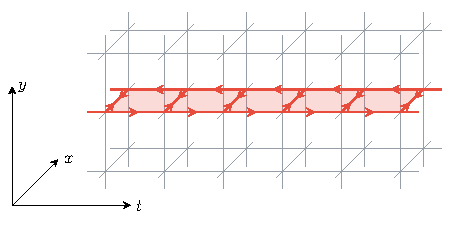
\includegraphics{Figs/puregauge1.pdf}}
    \only<2|handout:0>{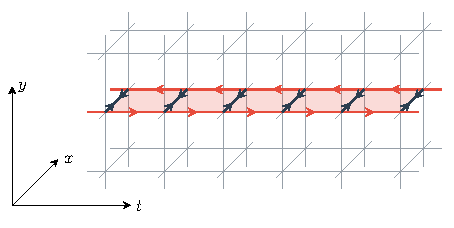
\includegraphics{Figs/puregauge2.pdf}}
    \only<3|handout:1>{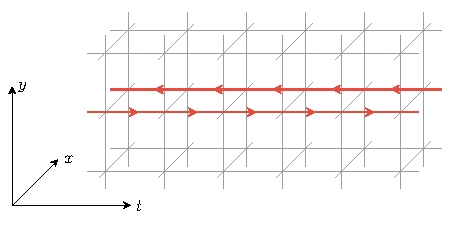
\includegraphics{Figs/puregauge3.pdf}}
  \end{center}

  \only<1|handout:0>{
    Put a strip of plaquettes in the time direction
  }
  \only<2|handout:0>{
    Integrate over all spatial gauge links
  }
  \only<3|handout:1>{
    What remains is an interaction between Polyakov Loops
  }
  
  \only<3|handout:1>{
  \nointerlineskip
  \begin{tikzpicture}[overlay, remember picture]
    \draw[<-,>=stealth] ([shift={(2.5,0.17)}] current page.center) .. controls +(.1,-.7) and +(-.3,0) .. +(2,-.4)
      node[scale=0.75,right] {$L$};
    \draw[<-,>=stealth] ([shift={(2.7,.62)}] current page.center) .. controls +(.1,.7) and +(-.3,0) .. +(2,+.4)
      node[scale=0.75,right] {$L^*$};
  \end{tikzpicture}
  }

\end{frame}

\begin{frame}
  \frametitle{Effective pure gauge theory}

  \begin{block}{Effective Gluon Interactions}
    \begin{equation*}
      S_{\mathrm{eff \: gluon}} \sim \lambda(\beta, N_t) \sum_{\langle x,y \rangle} L(x) L^*(y)
    \end{equation*}
  \end{block}

  \vspace{1em}

  \begin{center}
  \begin{tikzpicture}
    \draw[LightUIBase!50!white,use as bounding box] (-.3,-.3) grid[xstep=2] (6.3,2.3);
    \draw[thick,decorate, decoration={snake}, draw=LightUIBase] (2,1) -- (4,1)
      node[scale=0.75,midway,below=.2] {$\lambda$};
    \node[scale=2,fermion,fill=LightUIRed] at (4,1) (ell) {};
    \node[scale=0.75,above right=3pt of ell] {$L$};
    \node[scale=2,draw=LightUIRed, thick, circle, inner sep=0pt, minimum size=4pt] at (2,1) (elles) {};
    \node[scale=0.75,above left=3pt of elles] {$L^*$};

    \coordinate (coordcenter) at (-1,-1);
    \draw[->,>=stealth] (coordcenter) -- +(2,0) node[right,scale=0.75] {$x$};
    \draw[->,>=stealth] (coordcenter) -- +(0,2) node[right,scale=0.75] {$y$};
  \end{tikzpicture}
  \end{center}

  
\end{frame}

\begin{frame}
  \frametitle{Effective pure gauge theory}
  \framesubtitle{Higher order $\beta$ corrections}

  \begin{center}
    \includegraphics[width=\textwidth]{Figs/plaquette_correction.pdf}
  \end{center}

  Rescales $\lambda$:
  \[
    \lambda \to \lambda \Big( 1 + 4 N_t u(\beta)^4 \Big)
  \]

\end{frame}

\begin{frame}
  \frametitle{Lattice expansions}
  \framesubtitle{Hopping parameter expansion}

  One can rewrite the fermion matrix $\qmat$ as
  
  \vspace{2em}

  \begin{block}{}
    \[
      \det \qmat = \exp \bigg\{ - \sum_{n=1}^{\infty} \frac{1}{n} \kappa^n \tr H_{\mathrm{op}}^n \bigg\}
    \]
  \end{block}

  \vspace{1em}

  where $H_{\mathrm{op}}$ translates the quark one lattice spacing and \\ $\kappa \sim 1/m_q$


\end{frame}

\begin{frame}
  \frametitle{Spatial hopping expansion}

  \begin{center}
    \only<1|handout:0>{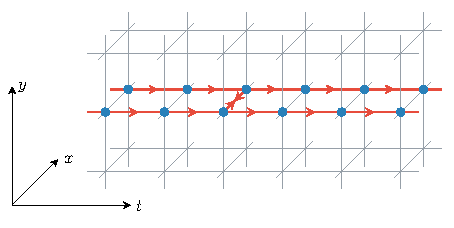
\includegraphics{Figs/purequark1.pdf}}
    \only<2|handout:0>{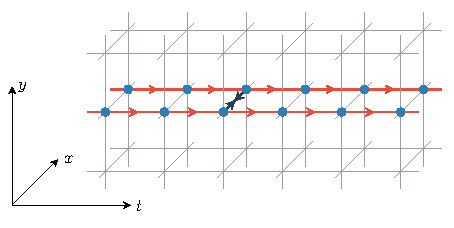
\includegraphics{Figs/purequark2.pdf}}
    \only<3|handout:1>{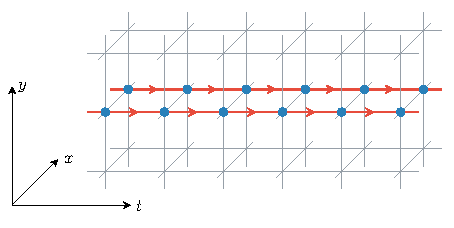
\includegraphics{Figs/purequark3.pdf}}
  \end{center}

  \begin{overlayarea}{\textwidth}{3em}
  \only<1|handout:0>{
    Can produce a closed quark loop with multiple temporal windings
  }
  \only<2|handout:0>{
    Once again integrate out spatial links
  }
  \only<3|handout:1>{
    Producing an interaction between the $W$ objects
  }
  \end{overlayarea}

  \only<3|handout:1>{
  \nointerlineskip
  \begin{tikzpicture}[overlay, remember picture]
    \node[scale=0.75] at ([shift={(5,.75)}] current page.center) (wNode) {$W[L]$};
    \draw[<-,>=stealth] ([shift={(2.5,.4)}] current page.center) .. controls +(.1,-.7) and +(-.3,0) .. ([yshift=-1] wNode.west);
    \draw[<-,>=stealth] ([shift={(2.9,1.)}] current page.center) .. controls +(.1,.7) and +(-.3,0) .. ([yshift=1] wNode.west);
  \end{tikzpicture}
  }
  
\end{frame}

\begin{frame}
  \frametitle{Spatial hopping expansion}

  \begin{block}{Effective Quark Interactions}
    \[
      S_{\mathrm{eff \: quarks}} \sim h_2(\kappa,N_t) \sum_{\langle x,y \rangle} W(x) W(y)
    \]
  \end{block}

  \vspace{1em}

  \begin{center}
  \begin{tikzpicture}
    \draw[LightUIBase!50!white,use as bounding box] (-.3,-.3) grid[xstep=2] (6.3,2.3);
    \draw[thick,decorate, decoration={snake}, draw=LightUIBase] (2,1) -- (4,1)
      node[scale=0.75,midway,below=.2] {$h_2$};
    \node[scale=2,draw=LightUIBlue, thick, circle, inner sep=0pt, minimum size=4pt] at (2,1) (w1) {};
    \node[scale=2,draw=LightUIBlue, thick, circle, inner sep=0pt, minimum size=4pt] at (4,1) (w2) {};
    \node[scale=0.75,above right=3pt of w2] {$W$};
    \node[scale=0.75,above left=3pt of w1] {$W$};

    \coordinate (coordcenter) at (-1,-1);
    \draw[->,>=stealth] (coordcenter) -- +(2,0) node[right,scale=0.75] {$x$};
    \draw[->,>=stealth] (coordcenter) -- +(0,2) node[right,scale=0.75] {$y$};
  \end{tikzpicture}
  \end{center}

\end{frame}

\begin{frame}
  \frametitle{Mixed contributions}

  \begin{block}{Correction to $\lambda$}
    \centering
    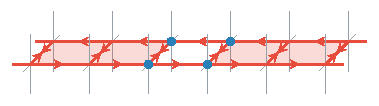
\includegraphics{Figs/lambdarenorm.pdf}
    \vspace*{-.5em}

  \begin{columns}
  \column{.35\textwidth}
  \begin{itemize}
    \item \color{LightUIBase} Rescales $\lambda$ 
  \end{itemize}
  \column{.35\textwidth}
  \begin{itemize}
    \item \color{LightUIBase} $\lambda \to \lambda(\kappa)$
  \end{itemize}
  \end{columns}
  \end{block}
  

  \begin{block}{Correction to $h_2$}
  \centering
  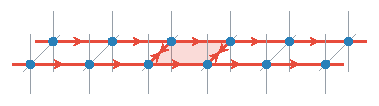
\includegraphics{Figs/h2renorm.pdf}
  \vspace*{-.5em}

  \begin{columns}
  \column{.35\textwidth}
  \begin{itemize}
    \item \color{LightUIBase} Rescales $h_2$ 
  \end{itemize}
  \column{.35\textwidth}
  \begin{itemize}
    \item \color{LightUIBase} $h_2 \to h_2(\beta)$
  \end{itemize}
  \end{columns}
  \end{block}
  
\end{frame}

\begin{frame}
  \frametitle{Spatially extended contributions}

  \only<1>{
  \begin{center}
    \includegraphics[scale=1.5]{Figs/plaquette_nnn.pdf}\par
    \begin{tikzpicture}
      \draw[->,>=stealth,line width=.6pt] (3,2.35) -- (3,1.65);
      \draw[LightUIBase!50!white,use as bounding box] (1.7,-.3) grid[xstep=2] (4.3,1.3);
      \draw[thick,decorate, decoration={snake}, draw=LightUIBase] (2,1) -- (4,0)
        node[scale=0.75,midway,above right=.2, yshift=-.2cm] {$\lambda_2$};
      \node[scale=2,fermion,fill=LightUIRed] at (4,0) (ell) {};
      \node[scale=0.75,below right=3pt of ell] {$L$};
      \node[scale=2,draw=LightUIRed, thick, circle, inner sep=0pt, minimum size=4pt] at (2,1) (elles) {};
      \node[scale=0.75,above left=3pt of elles] {$L^*$};
    \end{tikzpicture}
  \end{center}
  }

  \only<2>{
  \begin{center}
    \includegraphics[scale=1.5]{Figs/quark_eff_nnn.pdf}\par
    \begin{tikzpicture}
      \draw[->,>=stealth,line width=.6pt] (3,2.35) -- (3,1.65);
      \draw[LightUIBase!50!white,use as bounding box] (1.7,-.3) grid[xstep=2] (4.3,1.3);
      \draw[thick,decorate, decoration={snake, pre length=.2cm, post length=.2cm}, draw=LightUIBase] (2,1) -- (2,0);
      \draw[thick,decorate, decoration={snake, pre length=.2cm, post length=.15cm}, draw=LightUIBase] (2,0) -- (4,0);
      \node[scale=0.75] at (3,0.5) {$h_3$};
      \node[scale=2,draw=LightUIBlue, thick, circle, inner sep=0pt, minimum size=4pt] at (2,1) (w1) {};
      \node[scale=2,draw=LightUIBlue, thick, circle, inner sep=0pt, minimum size=4pt] at (4,0) (w2) {};
      \node[scale=2,draw=LightUIBlue, thick, circle, inner sep=0pt, minimum size=4pt] at (2,0) (w3) {};
      \node[scale=0.75,below right=3pt of w2] {$W$};
      \node[scale=0.75,above left=3pt of w1] {$W$};
      \node[scale=0.75,below left=3pt of w3] {$W$};
    \end{tikzpicture}
  \end{center}
  }
  
\end{frame}

\begin{frame}
  \frametitle{The effective lattice theory}

  \begin{alertblock}{The Effective Action}
    \[
      \mathcal{Z} = \int \prod_x \mathrm{d} L(x) \, \exp \big\{ \minus S_{\mathrm{eff \: action}} \big\}
    \]
    \[
      S_{\mathrm{eff \: action}} \sim \lambda \sum_{\langle x, y \rangle} L(x) L^*(y) + h_2\sum_{\langle x, y \rangle} W(x) W(y)
    \]
  \end{alertblock}

  \vspace{1em}

  The theory is contained in the set of coupling constants

  \[
    \lambda_1(\beta, N_t, \kappa), \lambda_2, ... \hspace{.5cm} h_1(\beta,N_t,\kappa), h_2, ...
  \]

\end{frame}

\begin{frame}
  \frametitle{Simulating the effective theory}

  The effective theory is numerically cheap to simulate

  \vspace{.5cm}

  \begin{itemize}
    \setlength\itemsep{.5em}
    \item No fermion determinant to calculate
    \item One dimension less
    \item Polyakov loop as only degree of freedom per site
    \item $N_t$ is only a parameter
  \end{itemize}

  \vspace{.5cm}

  Sign problem is mild \;$\Rightarrow$\; Reweighting works well
  
  
\end{frame}

\section{Analytic Calculations}
\sectionframe

\begin{frame}
  \frametitle{Motivation}

  {\centering
    \includegraphics[page=1, clip, trim=0 9.85cm 0 3cm, scale=0.7]{Figs/luscher_weisz_triviality.pdf}
    \par}

  
\end{frame}

\begin{frame}
  \frametitle{Similarity to the LCE}

  \begin{block}{$\lambda \phi^4$ theory}
    \[
      \int \prod \mathrm{d} \phi(x) \, \exp \bigg\{ -S_0[\phi] - \kappa \sum_{\langle x,y \rangle}
      \phi(x) \phi(y) \bigg\}
    \]
  \end{block}

  \vspace{.5cm}

  \begin{block}{Effective Theory}
    \[
      \int \prod \mathrm{d} L(x) \, \det Q^{\mathrm{stat}} \exp \bigg\{ \minus \lambda \sum_{\langle x, y \rangle} L(x) L^*(y) + ... \bigg\}
    \]
  \end{block}
  
\end{frame}

\begin{frame}
  \frametitle{Effective action as graphs}

  The theory contains interactions at all distances

  \vspace{.5em}

  \begin{block}{}
    \[
      S_I\big[ L \big] = \sum_{\vphantom{d}\mathrm{terms}} \sum_{\mathrm{dof}} v_i(1,2,...,n_i) \phi_1 \big[L\big] \phi_2 \big[L\big] \cdots
      \phi_{n_i} \big[ L \big]
    \]
  \end{block}

  \vspace{.5cm}

  {\color{LightUIRed} In our theory:}

  \vspace{.2cm}
  \begin{itemize}
    \setlength\itemsep{1em}
    \item $v_i(1,2,...n_i) \to \big\{ \lambda_i, h_i \big\} \times \mathrm{geometry}$
    \item $\phi_i \to \big\{ L_i, L_i^*, W_i \big\}$
  \end{itemize}
  
\end{frame}

\begin{frame}
  \frametitle{Graphs and embeddings}
  \framesubtitle{The N-point Linked Cluster Expansion}

  {\color{LightUIBlue}\large Classical Linked Cluster Expansion} \\[5pt]
  The action consists of two-point interactions which can be expanded in a set of connected graphs.

  \vspace{2em}

  {\color{LightUIBlue}\large Our Problem} \\[5pt]
  The action contains $n$-point interactions that we can embed on a set of connected graphs. \\[5pt]
  \hspace{1em}\tikz[baseline={-3pt},rounded corners=2pt] \draw[->,>=stealth] (0,.2) -- (0,0) -- (.5,0);
  Two step embedding
  
\end{frame}

\begin{frame}
  \frametitle{Graphs and embeddings}
  \framesubtitle{Two step embedding process}

  {\centering
    \begin{tikzpicture}
      \node[scale=0.75] (title1) {\strut{}Effective Action Term};
      \node[below=2pt of title1] (graphs1) {
\includegraphics{Graphs/graph1.pdf} \hspace{1em} 
\includegraphics{Graphs/graph2.pdf}};
      \node (fit1) [draw=LightUIBlue,rounded corners=2pt] [fit={(title1) (graphs1)}] {};

      \node[right=1.5cm of title1] (title2) [scale=0.75] {Skeleton Graph};
      \node[below=2pt of title2] (graphs2) [inner ysep=7.5pt] {\includegraphics{Graphs/graph_skel.pdf}};
      \node (fit2) [draw=LightUIBlue,rounded corners=2pt] [fit={(title2) (graphs2)}] {};

      \node (e1) at ([shift={(-2.2cm,-3cm)}] fit1.south) {\includegraphics{Graphs/graph_emb3.pdf}};
      \node[right=of e1] (e2) {\includegraphics{Graphs/graph_emb1.pdf}};
      \node[right=of e2] (e3) {\includegraphics{Graphs/graph_emb2.pdf}};
      \node[right=of e3] (e4) {\includegraphics{Graphs/graph_emb4.pdf}};

      \node (fit3) [draw=LightUIBlue,rounded corners=2pt] [fit={(e1) (e2) (e3) (e4)}] {};

      \coordinate (merge) at ([yshift=1.6cm] fit3.north);

      \draw[LightUIBlue,rounded corners=3pt] (fit1.south) |- (merge) -- (fit3.north);
      \draw[->,>=stealth,LightUIBlue,rounded corners=3pt] (fit2.south) |- (merge) -- (fit3.north)
        node[scale=0.75,text=LightUIBase,midway,right] {embedding};

    \end{tikzpicture}
  \par}
  
\end{frame}

\begin{frame}[plain]
  \begin{tikzpicture}[overlay,remember picture]
    \node[anchor=north] at ([shift={(0,.3)}] current page.north)
    {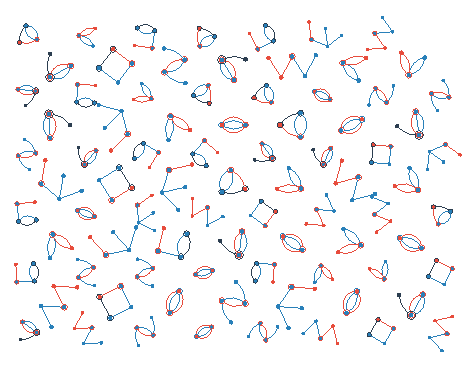
\includegraphics[scale=1.6]{Graphs/graphmatrix.pdf}};
  \end{tikzpicture}
\end{frame}

\begin{frame}
  \frametitle{Continuum comparison}

  {\centering
    \includegraphics[width=\textwidth]{Plots/nbVmu_comp.pdf}
  \par}

\end{frame}

\begin{frame}
  \frametitle{Two-step expansion}
  \framesubtitle{First expansion}

  {\centering
    \begin{tikzpicture}[node distance=.3cm, every node/.style={inner sep=0pt}]
      \node (strong) {Strong coupling expansion};
      \node[below=of strong] (plus) [LightUIRed,scale=1.5] {+};
      \node[below=of plus] (hopping) {Hopping parameter expansion};
      \draw[->,>=stealth,line width=1.2pt,LightUIRed] ([yshift=-.25cm] hopping.south) -- +(0,-.5cm);
    \end{tikzpicture}
  \par}

  \vspace*{-.25cm}

  \[
    \mathcal{Z} \approx \int \prod_x \mathrm{d} L(x) \, \exp \big\{ \minus S_{\mathrm{eff \: action}} \big\}
  \]
  \[
    S_{\mathrm{eff \: action}} =\sum_{n=0}^{N} \sum_{m=0}^{M} \kappa^n \beta^m S_{n,m} \tikzmark{effac}
  \]

  \nointerlineskip
  \begin{tikzpicture}[overlay,remember picture]
    \draw[line width=1.2pt,LightUIRed] ([shift={(.2cm, .5ex)}] effac) .. controls +(1.5cm,0) and +(0,2cm) ..
      ([xshift=-2cm] current page.south east);
  \end{tikzpicture}
  
\end{frame}

\begin{frame}
  \frametitle{Two-step expansion}
  \framesubtitle{Second expansion}

  \vspace{1cm}

  {\centering
    \begin{tikzpicture}[node distance=.3cm, every node/.style={inner sep=0pt},remember picture]
      \node (lce) {Linked cluster expansion};
      \draw[->,>=stealth,line width=1.2pt,LightUIRed] ([yshift=-.35cm] lce.south) -- +(0,-.5cm);
    \end{tikzpicture}
  \par}

  \vspace*{-.5cm}

  \begin{align*}
    \mathcal{W} &= -\frac{1}{\Omega} \log \mathcal{Z} \\
    &\approx \sum_{i,j} \sum_{n=0}^{N} \sum_{m=0}^{M} h_i^n \lambda_j^m W_{i,j,n,m} \\
    &\equiv \sum_{n=0}^{N_{\kappa}} \sum_{m=0}^{M_{\beta}} \kappa^n \beta^m W_{n,m}
  \end{align*}

  \nointerlineskip
  \begin{tikzpicture}[overlay,remember picture]
    \draw[->,>=stealth, line width=1.2pt,LightUIRed] ([xshift=-2cm] current page.north east) .. 
      controls +(0,-2cm) and +(0,2cm) .. ([yshift=.35cm] lce.north);
  \end{tikzpicture}
  
\end{frame}

\begin{frame}
  \frametitle{Analytic resummations}
  \framesubtitle{Extending the theory}

  Using the resummed Linked Cluster Expansion as motivation

  \vspace{2em}

  {\centering
    \includegraphics[scale=0.9]{Graphs/graph_renorm.pdf}
  \par}

  \vspace{2em}

  We can do the same resummation for the effective action itself, incorporating long-range effects
  
\end{frame}

\section{Results}
\sectionframe

\begin{frame}
  \frametitle{Convergence}

  {\centering%
    \only<1|handout:0>{\includegraphics[width=\textwidth]{Plots/resummed_conv_part1.pdf}}%
    \only<2|handout:0>{\includegraphics[width=\textwidth]{Plots/nucleon_compare_part1.pdf}}%
    \only<3|handout:1>{\includegraphics[width=\textwidth]{Plots/nucleon_compare_part2.pdf}}%
  \par}

  \begin{tikzpicture}[overlay,remember picture]
    \draw[->,>=stealth] ([shift={(2.5,1.15)}] current page.south) -- +(2,0)
      node[midway,below,scale=0.65] {$m_q \to 0$};
    \node[anchor=west] at ([shift={(-.7,-2.3)}] current page.north) [scale=0.8] {$h_1 = \kappa^{N_t} e^{N_t \mu} = 0.8$};
  \end{tikzpicture}

\end{frame}

\begin{frame}
  \frametitle{Effect of the resummations}

  {\centering%
    \only<1|handout:0>{\includegraphics[width=\textwidth]{Plots/resummed_conv_part2.pdf}}%
    \only<2|handout:1>{\includegraphics[width=\textwidth]{Plots/resummed_conv_part3.pdf}}%
  \par}

  \begin{tikzpicture}[overlay,remember picture]
    \draw[->,>=stealth] ([shift={(2.5,1.15)}] current page.south) -- +(2,0)
      node[midway,below,scale=0.65] {$m_q \to 0$};
    \node[anchor=west] at ([shift={(-.7,-2.3)}] current page.north) [scale=0.8] {$h_1 = \kappa^{N_t} e^{N_t \mu} = 0.8$};
  \end{tikzpicture}
\end{frame}

\begin{frame}
  \frametitle{Effect of the resummations}

  {\centering%
    \only<1|handout:0>{\includegraphics[width=\textwidth]{Plots/resummed_conv_part4.pdf}}%
    \only<2|handout:0>{\includegraphics[width=\textwidth]{Plots/resummed_conv_part5.pdf}}%
    \only<3|handout:1>{\includegraphics[width=\textwidth]{Plots/resummed_conv_part6.pdf}}%
  \par}

  \begin{tikzpicture}[overlay,remember picture]
    \draw[->,>=stealth] ([shift={(2.5,1.15)}] current page.south) -- +(2,0)
      node[midway,below,scale=0.65] {$m_q \to 0$};
    \node[anchor=west] at ([shift={(-.7,-2.3)}] current page.north) [scale=0.8] {$h_1 = \kappa^{N_t} e^{N_t \mu} = 1.0$};
  \end{tikzpicture}
\end{frame}

\begin{frame}
  \frametitle{Attempts at the binding energy}

  {\centering
    \includegraphics[width=\textwidth]{Plots/binding_energy.pdf}
  \par}

  \begin{tikzpicture}[overlay,remember picture]
    \node[text=LightUIBase,scale=0.75] at ([shift={(1,-2)}] current page.north) [anchor=west] {$\epsilon = \displaystyle\frac{e - m_B n_B}{m_B n_B}$};
  \end{tikzpicture}

\end{frame}

\begin{frame}
  \frametitle{Towards lighter quarks}

  {\centering
    \includegraphics[width=\textwidth]{Plots/nbOfPi_T10_a01.pdf}
  \par}
  
\end{frame}

\begin{frame}
  \frametitle{Towards lighter quarks}

  {\centering
    \includegraphics[width=\textwidth]{Plots/nbOfPi_T20_a02.pdf}
  \par}
  
\end{frame}

\begin{frame}
  \frametitle{Equation of state}

  {\centering
    \includegraphics[width=\textwidth]{Plots/nbVpress_w_fit.pdf}
  \par}
  
\end{frame}

\section{Conclusion}
\sectionframe

\begin{frame}
  \frametitle{Summary}

  {\color{LightUIRed} Summary}

  \vspace{.2cm}
  \begin{itemize}
    \setlength\itemsep{1em}
    \item Introduced the effective dimensionally reduced lattice theory
    \item Looked at how a consistent analytic calculation could be carried out
    \item Demonstrated convergence and comparisons with numerics
  \end{itemize}
  
\end{frame}

\begin{frame}
  \frametitle{Outlook}

  {\color{LightUIRed} Outlook}

  \vspace{.2cm}
  \begin{itemize}
    \setlength\itemsep{1em}
    \item Use the analytic results as a tool to study the characteristics of the effective theory
    \item Find analytic resummation schemes to incorporate long-range effects
  \end{itemize}
  
\end{frame}


\end{document}
